%!TEX root = main.tex

Although technically any characterization result finds the exact value of the extrema of a function, computationally this is hardly feasible (specially for functions of very high dimension).  See the following session based on problem \ref{problem:tricky} for an example, where we try to find the critical points of the function $f(x,y,z)=e^{x^2+y^2+z^2}-x^4-y^y-z^6$ symbolically in Python with the \texttt{sympy} libraries:

% framesep=2mm,
% baselinestretch=1.2,
\begin{minted}[frame=single, fontsize=\footnotesize, linenos ]{python}
# Importing necessary symbols/libraries/functions
from sympy.abc import x,y,z
from sympy import Matrix, solve, exp
from sympy.tensor.array import derive_by_array

# Description of f, computation of its gradient and Hessian
f = exp(x**2 + y**2 + z**2) - x**4 -y**6 - z**6
gradient = derive_by_array(f, [x,y,z])
hessian  = Matrix([derive_by_array(gradient, a) for a in [x,y,z]])
\end{minted}
While the correct expressions for $\gradient{f}$ and $\Hess{f}$ are quickly computed, trying to find critical points results in an error:
\begin{minted}[frame=single,fontsize=\footnotesize,mathescape]{python}
>>> solve(gradient) # Search of critical points by solving $\gradient{f}=0$
NotImplementedError: could not solve 
4*x**2*sqrt(-log(exp(x**2)/(2*x**2))) - 6*(-log(exp(x**2)/(2*x**2)))**(5/2)
\end{minted}

Too complex a task to be performed symbolically, although the obvious answer is $(0,0,0)$.  A better way to approach this is by trying to approximate this minimum using the structure of the graph of $f$.  In these notes we are going to explore several strategies to accomplish this task, based on the concept of \emph{iterative methods for finding zeros of real-valued functions}.

\section{Newton-Raphson's Method}\index{Newton method|see {Newton-Raphson method}}

\subsection{Newton-Raphson Method to search for roots of univariate functions}

In order to find a good estimation of $\sqrt{2}$ with many decimal places, we allow a computer to find better and better approximations of the root  of the polynomial $p(x)=x^2-2$.  We start with an initial guess, say $x_0=3$.  We construct a sequence $\{ x_n \}_{n\in\field{N}}$ that converges to $\sqrt{2}$ as follows:
\begin{enumerate}
\item Find the tangent line to the graph of $p$ at $x_0$, 
\begin{equation*}
y = p(x_0) + p'(x_0)(x-x_0)
\end{equation*}
Intuitively, we \emph{substitute} the original function $f$ by the approximation given by the derivative.  It is so much easier to seek roots of this simpler function, and that is what we do to \emph{approximate} the roots of $p$.
\item Provided the corresponding line is not horizontal ($p'(x_0)\neq 0$), report the intersection of this line with the $x$--axis.  Call this intersection $x_1$
\begin{equation*}
p'(x_0) (x_1 - x_0) = -p(x_0)
\end{equation*}
or equivalently,
\begin{equation*}
x_1=x_0-\frac{p(x_0)}{p'(x_0)}
\end{equation*}
\item Repeat this process, to get a sequence 
\begin{equation*}
x_{n+1} = x_n - \frac{p(x_n)}{p'(x_n)} = x_n - \frac{x_n^2-2}{2x_n}=\frac{x_n}{2}-\frac{1}{x_n}.
\end{equation*}
\end{enumerate}
\begin{figure}[ht!]
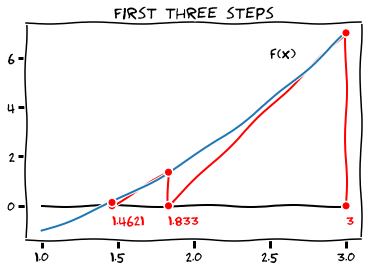
\includegraphics[width=0.6\linewidth]{images/newton1.png}
\caption{Newton-Raphson iterative method}
\label{figure:Newton-Raphson}
\end{figure}
Note the result of applying this process a few times:
\begin{center}\label{table:Newton-Raphson}
% \begin{table}[ht!]
\begin{tabular}{|c|c|r|} \hline 
$n$ & $x_n$ & $p(x_n)$ \\ \hline \hline 
$0$ & $3.000000000000000$ & $7.0000E+00$ \\ \hline 
$1$ & $1.833333333333333$ & $1.3611E+00$ \\ \hline 
$2$ & $1.462121212121212$ & $1.3780E-01$ \\ \hline 
$3$ & $1.414998429894803$ & $2.2206E-03$ \\ \hline 
$4$ & $1.414213780047198$ & $6.1568E-07$ \\ \hline 
$5$ & $1.414213562373112$ & $4.7518E-14$ \\ \hline 
$6$ & $1.414213562373095$ & $-4.4409E-16$ \\ \hline 
$7$ & $1.414213562373095$ & $4.4409E-16$ \\ \hline 
\end{tabular}
% \caption{Newton-Raphson method: Convergence to $\sqrt{2}$ with 15-digit accuracy in 6 steps}
% \end{table}
\end{center}

\begin{definition}\index{Newton-Raphson method!iteration}\index{Newton-Raphson method}\index{Newton-Raphson method!recursive formula}
Given a differentiable real-valued function $f\colon \field{R} \to \field{R}$ and an initial guess $x_0 \in \field{R}$, we define the \emph{Newton-Raphson iteration} to be the sequence $\{ x_n \}_{n \in \field{N}}$ given by one of the two following \emph{recursive formulas}
\begin{equation}\label{equation:NewtonRaphson1dim}
\begin{split}
f'(x_n) (x_{n+1}-x_n) = -f(x_n) \\
x_{n+1} = x_n - \frac{f(x_n)}{f'(x_n)}
\end{split}
\end{equation}
The \emph{Newton-Raphson method} (or \emph{Newton method}) refers to employing this sequence to search and approximate roots of the equation $f(x) = 0$.
\end{definition}

\begin{example}\label{example:NewtonRaphsonChoice}
Consider now the function $f(x) = 1-\tfrac{1}{x}$ over $(0, \infty)$, which has the obvious root $x=1$. The Newton-Raphson method gives the following iterates for any $x_0 \in (0,\infty)$:
\begin{align*}
x_{n+1} = x_n - \frac{f(x_n)}{f'(x_n)} = x_n \big( 2- x_n \big).
\end{align*}
Notice the two factors in the right-hand side of that expression: $x_n$, and $2-x_n$.  If the initial guess does not satisfy $0<x_0<2$, then the next iteration gives a non-positive value (see Figure \ref{figure:NewtonRaphsonChoice}).  The method will not work on those instances: convergence to a solution is not guaranteed.
\begin{figure}[ht!]
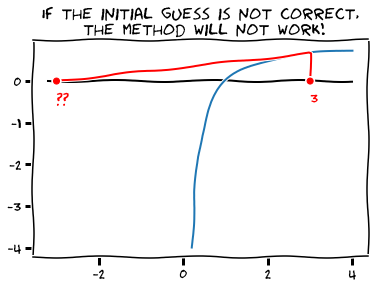
\includegraphics[width=0.55\linewidth]{images/badNewton.png}
\caption{Initial guess must be carefully chosen in Newton-Raphson}
\label{figure:NewtonRaphsonChoice}
\end{figure}
\end{example}

\begin{example}\label{example:NewtonRaphsonloop}
Consider now $f(x) = \sign(x)\sqrt{\lvert x \rvert}$ over $\field{R}$, with root at $x=0$.  The Newton-Raphson method fails miserably with this function: for any $x_0 \neq 0$
\begin{align*}
x_1 = x_0 - \frac{f(x_0)}{f'(x_0)} = x_0 - \frac{\sign(x_0)\lvert x_0 \rvert^{1/2}}{\tfrac{1}{2}\lvert x_0 \rvert^{-1/2}} = -x_0.
\end{align*}
This sequence turns into a loop: $x_{2n}=x_0$, $x_{2n+1}=-x_0$ for all $n\in \field{N}$ (see Figure \ref{figure:NewtonRaphsonloop}).
\begin{figure}[ht!]
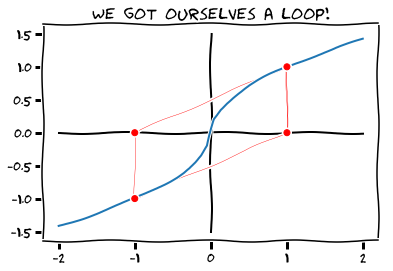
\includegraphics[width=0.55\linewidth]{images/loop.png}
\caption{Newton-Raphson fails for some functions}
\label{figure:NewtonRaphsonloop}
\end{figure}
\end{example}

\subsection{Efficiency of Newton-Raphson's Method}\index{Newton-Raphson method!error}
To study the error in a Newton-Raphson iteration $\{ x_n \}_{n \in \field{N}}$ that converges to a root $x^\star$ of the function $f$, we observe that
\begin{align}
x_{n+1} - x^\star &= x_n - x^\star - \frac{f(x_n)}{f'(x_n)} \nonumber \\
&= (x_n - x^\star) \bigg( 1 - \frac{f(x_n)-\overbrace{f(x^\star)}^0}{(x_n-x^\star)f'(x_n)} \bigg) \nonumber \\
&= (x_n - x^\star) \bigg( 1 - \frac{1}{f'(x_n)} \frac{f(x_n) - f(x^\star)}{x_n - x^\star} \bigg) \label{eq:NRestimateStandBy}
\end{align}
Recall at this point the definition of \emph{divided differences} for any $n$--times differentiable function $g\colon \field{R} \to \field{R}$, and a family of values $t_0 \leq t_1 \leq \dotsb \leq t_n$:\index{Divided differences}
\begin{align*}
\Delta g[t_0,t_1] &= \frac{g(t_1)-g(t_0)}{t_1-t_0} \qquad\text{ (if }t_0 \neq t_1)\\
\Delta g[t_0,t_0] &= g'(t_0) \\
\Delta g[t_0,t_1,\dotsc,t_n] &= \frac{\Delta g[t_1, t_2, \dotsc, t_n] - \Delta g[t_0, t_1, \dotsc, t_{n-1}]}{t_n-t_0} \quad\text{(if }t_0 \neq t_n)\\
\Delta g[\underbrace{t_0, \dotsc, t_0}_{n+1 \text{ times}}] &= \frac{1}{n!} g^{(n)}(t_0) \qquad \text{(Why? \textbf{Hint:} Taylor's Polynomial)}
\end{align*}
We can then rewrite \eqref{eq:NRestimateStandBy} in terms of divided differences as follows:
\begin{align*}
x_{n+1} - x^\star &= (x_n - x^\star) \bigg( 1 - \frac{\Delta f[x_n, x^\star]}{\Delta f[x_n, x_n]}  \bigg) \\
&= (x_n - x^\star) \frac{ \Delta f[x_n, x_n] - \Delta f[x_n, x^\star] }{\Delta f [x_n,x_n]} \\
&= (x_n - x^\star) \frac{ \Delta f[x_n, x_n] - \Delta f[x_n, x^\star] }{x_n - x^\star} \frac{ x_n - x^\star }{\Delta f [x_n,x_n]} \\
& =(x_n - x^\star)^2 \frac{\Delta f[x_n, x_n, x^\star]}{\Delta f[x_n, x_n]}
\end{align*}
Therefore, 
\begin{equation*}
\lim_n \frac{x_{n+1}-x^\star}{(x_n - x^\star)^2} = \lim_n \frac{\Delta f[x_n, x_n, x^\star]}{\Delta f[x_n, x_n]} 
= \frac{f''(x^\star)}{2f'(x^\star)}.
\end{equation*}
If $f''(x^\star) \neq 0$, the Newton-Raphson's iteration exhibits quadratic convergence.\footnote{See Appendix \ref{appendix:convergence}}

\begin{remark} 
We have just proven that, if a Newton-Raphson iteration for a function $f$ gives a convergent sequence, the convergence is quadratic.  But, how can we guarantee convergence to a root of $f$?  The key is in \emph{how far can we start the sequence} given the structure of the graph of $f$.
\end{remark}

\begin{theorem}[Local Convergence for the Newton-Raphson Method]\label{theorem:LCNR}\index{Newton-Raphson method!Local convergence for}\index{Theorem!Local Convergence for Newton-Raphson}
Let $x^\star$ be a simple root of the equation $f(x)=0$, and assume that there exists $\varepsilon > 0$ so that 
\begin{itemize}
	\item $f$ is twice continuously differentiable in the interval $(x^\star-\varepsilon, x^\star + \varepsilon)$, and
	\item there are no critical points of $f$ on that interval.
\end{itemize}  
Set
\begin{equation*}
M(\varepsilon) = \max \bigg\{ \bigg\lvert \frac{f''(s)}{2f'(t)} \bigg\rvert : x^\star -\varepsilon < s,t < x^\star + \varepsilon \bigg\}.
\end{equation*}
If $\varepsilon$ is small enough so that $\varepsilon M(\varepsilon) < 1$, then 
\marginnote{I have seen this Theorem in \cite{gautschi2011numerical} with the condition $2 \varepsilon M(\varepsilon) < 1$ instead, but I could not see why that 2 was necessary.  What am I missing?}
\begin{enumerate}
	\item \label{thm:LCNR1} There are no other roots of $f$ in $(x^\star -\varepsilon, x^\star+\varepsilon)$.
	\item \label{thm:LCNR2} Any Newton-Raphson iteration starting at an initial guess $x_0 \neq x^\star$ in that interval will converge (quadratically) to $x^\star$
\end{enumerate} 
\end{theorem}
\begin{proof}
Start with Taylor's Theorem for $f$ around $x^\star$.  Given $x\neq x^\star$ satisfying $\abs{x-x^\star} < \varepsilon$, there exists $\xi$ between $x$ and $x^\star$ so that
\begin{align*}
f(x) &= f(x^\star) + (x-x^\star) f'(x^\star) + \tfrac{1}{2}(x-x^\star)^2 f''(\xi) \\
&= (x-x^\star)f'(x^\star) \bigg( 1 + (x-x^\star) \frac{f''(\xi)}{2f'(x^\star)} \bigg)
\end{align*}
Note that the three factors on the last expression are never zero:
\begin{align*}
x-x^\star &\neq 0 &&\text{(since }x \neq x^\star\text{ by hypothesis)} \\
f'(x^\star) &\neq 0 &&\text{(no critical points by hypothesis)} \\
\bigg\lvert (x-x^\star) \frac{f''(\xi)}{2f'(x^\star)} \bigg\rvert &\leq \varepsilon M(\varepsilon) < 1 &&\text{(by hypothesis on }M(\varepsilon))
\end{align*}
This proves \ref{thm:LCNR1}.

We want to prove now that all terms of a Newton-Raphson iteration stay in the interval $(x^\star - \varepsilon, x^\star + \varepsilon)$. We do that by induction:
\begin{itemize}
	\item $\abs{x_0 - x^\star}<\varepsilon$ by hypothesis.
	\item Assume $\abs{x_n-x^\star} < \varepsilon$.  In that case,
	\begin{equation*}
	\big\lvert x_{n+1} - x^\star \big\rvert = \big\lvert x_n - x^\star \big\rvert^2 \bigg\lvert \frac{\Delta f[x_n, x_n, x^\star]}{\Delta f[x_n, x_n]} \bigg\rvert
	\end{equation*}	
	but $\Delta f [x_n, x_n] = f'(x_n)$, and there exist $\xi_n$ between $x_n$ and $x^\star$ so that $\Delta f[x_n,x_n,x^\star] = \tfrac{1}{2}f''(\xi_n)$; therefore,
	\begin{equation*}
	\big\lvert x_{n+1} - x^\star \big\rvert = \big\lvert x_n - x^\star \big\rvert^2 \bigg\lvert \frac{f''(\xi)}{2f'(x_n)} \bigg\rvert \leq \varepsilon^2 M(\varepsilon) = \varepsilon \cdot \varepsilon M(\varepsilon) < \varepsilon.
	\end{equation*}
\end{itemize}
The next step is to prove that there is convergence.  A similar computation to the previous gives
\begin{equation*}
\big\lvert x_n - x^\star \big\rvert \leq \varepsilon M(\varepsilon) \big\lvert x_{n-1} - x^\star \big\rvert \leq \big( \varepsilon M(\varepsilon) \big)^n \big\lvert x_0 - x^\star \big\rvert.
\end{equation*}
Since $\varepsilon M(\varepsilon) < 1$, $\lim_n \big( \varepsilon M(\varepsilon) \big)^n = 0$, and $\{ x_n \}_{n \in \field{N}}$ converges to $x^\star$.
\end{proof}

\begin{example}
Let's use this Theorem to prove convergence of Newton-Raphson iterations for $f(x)= x^2-2$ for initial guesses $x_0$ in a meaningful interval---something like the obvious choice $x_0 \in [1,2]$.  Pick for example $\varepsilon = \sqrt{2}/2$, so we can analyze convergence with initial guesses in the interval $[\sqrt{2}/2, 3\sqrt{2}/2] \supset [1,2]$.  Note that
\begin{align*}
M\big(\tfrac{\sqrt{2}}{2}\big) &= \max \bigg\{ \frac{1}{2t} : \frac{\sqrt{2}}{2} < t < \frac{3\sqrt{2}}{2} \bigg\} = \frac{\sqrt{2}}{2} \\
\intertext{and thus,}
\varepsilon M(\varepsilon) &= \frac{\sqrt{2}}{2} M\big(\tfrac{\sqrt{2}}{2}\big) = \frac{1}{2} < 1.
\end{align*}
By virtue of Theorem \ref{theorem:LCNR} we have quadratic convergence to $\sqrt{2}$ if we start with any initial guess in this interval.
\end{example}

\subsection{Extension to higher dimensions}

Let's proceed to extend this process to functions $\boldsymbol{g} \colon \field{R}^d \to \field{R}^d$ as follows.
\begin{itemize}
	\item Any function $\boldsymbol{g} \colon \field{R}^d \to \field{R}^d$ can be described in the form $\boldsymbol{g}(\x) = \big[ g_1(\x), g_2(\x), \dotsc, g_d(\x) \big]$ for $d$ real-valued functions $g_k\colon \field{R}^d \to \field{R}$ ($1\leq k \leq d$).
	\item For such a function $\boldsymbol{g}$, the \emph{derivative} is the Jacobian
	\begin{equation*}
	\boldsymbol{J} \boldsymbol{g} = \gradient{\boldsymbol{g}} = \begin{bmatrix}
	\frac{\partial g_1}{\partial x_1} & \frac{\partial g_1}{\partial x_2} & \dotsb & \frac{\partial g_1}{\partial x_d} \\ \\
	\frac{\partial g_2}{\partial x_1} & \frac{\partial g_2}{\partial x_2} & \dotsb & \frac{\partial g_2}{\partial x_d} \\ \\
	\vdots & \vdots & \ddots & \vdots \\ \\
	\frac{\partial g_d}{\partial x_1} & \frac{\partial g_d}{\partial x_2} & \dotsb & \frac{\partial g_d}{\partial x_d} \\
	\end{bmatrix}
	\end{equation*}
\end{itemize}
Start with a guess for the solution, $\x_0$.  As we did in the one-dimensional case, we \emph{substitute} the function $\boldsymbol{g}$ by the linear approximation given by the Jacobian:
\begin{equation*}
\transpose{\y} = \transpose{\boldsymbol{g}(\x_0)}+ \gradient{\boldsymbol{g}}\transpose{(\x_0)(\x - \x_0)}.
\end{equation*}
Provided the determinant of the Jacobian $\gradient{\boldsymbol{g}}$ is not zero, there is only one solution for the equation $\y = \boldsymbol{0}$.
 The computation of $\x_1$ is therefore the solution of the following system of linear equations:
\begin{equation*}
\gradient{\boldsymbol{g}}\transpose{(\x_0)(\x_1-\x_0)} = -\transpose{\boldsymbol{g}(\x_0)}, 
\end{equation*}
or equivalently,
\begin{equation*}
\transpose{\x_1} = \transpose{\x_0} - \big[ \gradient{\boldsymbol{g}}(\x_0) \big]^{-1} \cdot \transpose{\boldsymbol{g}(\x_0)}.
\end{equation*}
We iterate this process to obtain a sequence of approximations $\{ \x_n \}_{n \in \field{N}}$ to a root, via any of the following two recursive formulas:
\begin{equation}\label{equation:NewtonMethod}
\begin{split}
\gradient{\boldsymbol{g}}(\x_n) \transpose{(\x_{n+1}-\x_n)} = -\transpose{\boldsymbol{g}(\x_n)}, \\
\transpose{\x_{n+1}} = \transpose{\x_n} - \big[ \gradient{\boldsymbol{g}}(\x_n) \big]^{-1} \cdot \transpose{\boldsymbol{g}(\x_n)},
\end{split}
\end{equation}
\index{Newton-Raphson method}
\index{Newton-Raphson method!iteration}
\index{Newton-Raphson method!recursive formula}

\begin{example}\label{example:preNewton4poly4}
Consider the function $\boldsymbol{g}\colon \field{R}^2 \to \field{R}^2$ given by
\begin{equation*}
\boldsymbol{g}(x,y,z) = \big[ x^3-y, y^3-x \big]
\end{equation*}
Its Jacobian at each $(x,y)$ is given by
\begin{equation*}
\gradient{\boldsymbol{g}}(x,y) = \begin{bmatrix} 3x^2 & -1 \\ -1 & 3y^2 \end{bmatrix}
\end{equation*}
Note the determinant of this matrix is $\det \gradient{\boldsymbol{g}}(x,y) = 9x^2y^2-1 = (3xy-1)(3xy+1)$.  For any point $(x,y)$ that does not make this expression zero, this is an invertible matrix with 
\begin{equation*}
\big[ \gradient{\boldsymbol{g}}(x,y)\big]^{-1} = \frac{1}{9x^2y^2-1}\begin{bmatrix} 3y^2 & 1 \\ 1 & 3x^2 \end{bmatrix}
\end{equation*}
For an initial guess $(x_0, y_0)$, the sequence computed by this method is then given by
\begin{align*}
\begin{bmatrix} x_{n+1} \\ y_{n+1} \end{bmatrix} &= \begin{bmatrix} x_n \\ y_n \end{bmatrix} -\frac{1}{9 x_n^2 y_n^2-1}\begin{bmatrix} 3y_n^2 & 1 \\ 1 & 3x_n^2 \end{bmatrix} \begin{bmatrix} x_n^3-y_n \\ y_n^3-x_n \end{bmatrix} \\
% &= \begin{bmatrix}
% x_n - \frac{3x_n^3 y_n^2-2 y_n^3-x_n}{9x_n^2  y_n^2-1} \\  y_n - \frac{3x_n^2 y_n^3+-2x_n^3- y_n}{9x_n^2 y_n^2-1}
% \end{bmatrix}
\end{align*}
Let's run this process with three different initial guesses:
\begin{enumerate}
	\item Starting at $(x_0, y_0) = (-1.0,1.0)$, the sequence converges to $(0,0)$.  %See Table \ref{table:00}.
	\begin{center}
	% \begin{table}[ht!]
	\begin{tabular}{|c|c|c|} \hline 
	$n$ & $x_n$ & $y_n$ \\ \hline \hline 
	$0$ & $-1.00000000$ & $1.00000000$ \\ \hline 
	$1$ & $-0.50000000$ & $0.50000000$ \\ \hline 
	$2$ & $-0.14285714$ & $0.14285714$ \\ \hline 
	$3$ & $-0.00549451$ & $0.00549451$ \\ \hline 
	$4$ & $-0.00000033$ & $0.00000033$ \\ \hline 
	$5$ & $-0.00000000$ & $0.00000000$ \\ \hline 
	$6$ & $-0.00000000$ & $0.00000000$ \\ \hline 
	\end{tabular}
	% \caption{Newton Method: Convergence to $(0,0)$ with 8-digit accuracy in 5 steps}
	% \label{table:N00}
	% \end{table}
	\end{center}
	\item Starting at $(x_0,y_0) = (3.5, 2.1)$, the sequence converges to $(1,1)$.  %See Table \ref{table:11}.
	\begin{center}
	% \begin{table}[ht!]
	\begin{tabular}{|c|c|c|} \hline 
	$n$ & $x_n$ & $y_n$ \\ \hline \hline 
	$0$ & $3.50000000$ & $2.10000000$ \\ \hline 
	$1$ & $2.37631607$ & $1.57961573$ \\ \hline 
	$2$ & $1.65945969$ & $1.27476534$ \\ \hline 
	$3$ & $1.23996276$ & $1.10419072$ \\ \hline 
	$4$ & $1.04837462$ & $1.02274752$ \\ \hline 
	$5$ & $1.00260153$ & $1.00133122$ \\ \hline 
	$6$ & $1.00000824$ & $1.00000451$ \\ \hline 
	$7$ & $1.00000000$ & $1.00000000$ \\ \hline 
	$8$ & $1.00000000$ & $1.00000000$ \\ \hline 
	\end{tabular}
	% \caption{Newton Method: Convergence to $(1,1)$ with 8-digit accuracy in 7 steps}
	% \label{table:N11}
	% \end{table}
	\end{center}
	\item Starting at $(x_0, y_0) = (-13.5, -7.3)$, the sequence converges to $(-1,-1)$.  %See Table \ref{table:-1-1}.
	\begin{center}
	% \begin{table}[ht!]
	\begin{tabular}{|c|c|c|} \hline 
	$n$ & $x_n$ & $y_n$ \\ \hline \hline 
	$0$ & $-13.50000000$ & $-7.30000000$ \\ \hline 
	$1$ & $-9.00900415$ & $-4.92301873$ \\ \hline 
	$2$ & $-6.01982204$ & $-3.36480659$ \\ \hline 
	$3$ & $-4.03494126$ & $-2.36199873$ \\ \hline 
	$4$ & $-2.72553474$ & $-1.73750959$ \\ \hline 
	$5$ & $-1.87830623$ & $-1.36573112$ \\ \hline 
	$6$ & $-1.36121191$ & $-1.15374930$ \\ \hline 
	% \end{tabular}~\begin{tabular}{|c|c|c|} \hline
	% $n$ & $x_n$ & $y_n$ \\ \hline \hline 
	$7$ & $-1.09518303$ & $-1.04341362$ \\ \hline 
	$8$ & $-1.00932090$ & $-1.00463507$ \\ \hline 
	$9$ & $-1.00010404$ & $-1.00005571$ \\ \hline 
	$10$ & $-1.00000001$ & $-1.00000001$ \\ \hline 
	$11$ & $-1.00000000$ & $-1.00000000$ \\ \hline 
	$12$ & $-1.00000000$ & $-1.00000000$ \\ \hline 
	$13$ & $-1.00000000$ & $-1.00000000$ \\ \hline 
	\end{tabular}
	% \caption{Newton Method: Convergence to $(-1,-1)$ with 8-digit accuracy in 11 steps}
	% \label{table:N-1-1}
	% \end{table}
	\end{center}
\end{enumerate}
\end{example}

\begin{remark}
The Newton-Raphson's method to solve $\boldsymbol{g}=\boldsymbol{0}$, as given by the recursive formula with the inverse of the gradient is very convenient to provide explicit descriptions of the different iterations.  However, it is hardly suitable for practical purposes, due to the computational issues involving matrix inversion.\index{Matrix!inversion}\index{Matrix!inverse}

To avoid dealing with matrix inversion, we exclusively use the equivalent formula $\gradient{\boldsymbol{g}}(\x_n) \transpose{\big( \x_{n+1} - \x_n \big)} = -\transpose{\boldsymbol{g}(\x_n)}$, since it offers a simple system of linear equations, which is a much more reliable process, prone to less numerical error.
\end{remark}

\subsection{Optimization via Newton's Method}
We can readily see how this process aids in the computation of critical points of twice continuously differentiable real-valued function $f\colon \field{R}^d \to \field{R}$:
\begin{enumerate}
	\item Set $\boldsymbol{g}(\x) = \gradient{f}(\x) = \big[ \frac{\partial f}{\partial x_1}, \dotsc, \frac{\partial f}{\partial x_d} \big]$
	\item It is then $\gradient{\boldsymbol{g}}(\x) = \Hess{f}(\x)$
	\item Perform a Newton method (with initial guess $\x_0$) on $\boldsymbol{g}=\gradient{f}$ to obtain the recursive formula
	\begin{equation}\label{equation:Newton4Crit}
	\transpose{\x_{n+1}} = \transpose{\x_n} - \big[ \Hess{f}(\x_n) \big]^{-1} \cdot \transpose{\gradient{f}(\x_n)}
	\end{equation}
\end{enumerate}

\begin{example}\label{example:NewtonPoly4}
Consider the polynomial $p_4(x,y) = x^4-4xy+y^4$. Notice $\gradient{p_4}(x,y) = \big[ x^3-y, y^3-x \big]$---this is function $\boldsymbol{g}$ in Example \ref{example:preNewton4poly4}.  The critical points we found were $(0,0)$, $(-1,-1)$ and $(1,1)$.  See Figure \ref{figure:NewtonConvergence}.
\end{example}
\begin{example}
A similar process for the Rosenbrock function\index{Function!Rosenbrock}\index{Function!Rosenbrock}
\begin{equation*}
\mathcal{R}_{1,1}(x,y) = (1-x)^2 + (y-x^2)^2
\end{equation*}
gives the following recursive formula:
\begin{align*}
\begin{bmatrix} x_{n+1} \\ y_{n+1} \end{bmatrix} &=
\begin{bmatrix} x_{n} \\ y_{n} \end{bmatrix} - \big[ \Hess{\mathcal{R}_{1,1}}(x_n,y_n) \big]^{-1} \cdot \transpose{\gradient{\mathcal{R}_{1,1}}(x_n, y_n)} \\
% &= \begin{bmatrix} x_{n} \\ y_{n} \end{bmatrix} - \tfrac{2}{2x^2-2y+1} \begin{bmatrix}
% 1/2 & x_n \\ x_n & 6x_n^2-2y_n+1
% \end{bmatrix} \begin{bmatrix}
% 2x_n^3-2x_n y_n +x_n -1 \\ y_n -x_n^2
% \end{bmatrix} \\
&= \frac{1}{2x_n^2-2y_n+1} \begin{bmatrix}
2x_n^3-2x_n y_n+1 \\ x_n(2x_n^3-2x_n y_n-x_n+2)
\end{bmatrix}
\end{align*}
For instance, starting with the initial guess $(x_0, y_0) = (-2,2)$, the sequence converges to the critical point $(1,1)$ in a few steps.  See Figure \ref{figure:NewtonConvergence}.
\end{example}
\begin{figure}[ht!]
\begin{tabular}{cc}
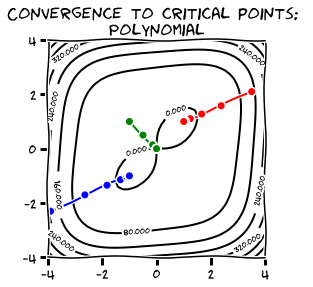
\includegraphics[width=0.45\linewidth]{images/convergenceNewton.png} &
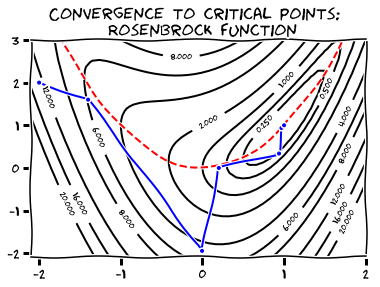
\includegraphics[width=0.55\linewidth]{images/convergenceNewtonRosenbrock.png} 
\end{tabular}
\caption{Newton-Raphson method}
\label{figure:NewtonConvergence}
\end{figure}

\begin{remark}
The equivalent recursive formula to \eqref{equation:Newton4Crit} to search for critical points of a twice continuously differentiable real-valued function $f \colon \field{R}^d \to \field{R}$ is given by
\begin{equation}\index{Newton-Raphson method}\index{Newton-Raphson method!recursive formula}\index{Newton-Raphson method!iteration}\index{Newton-Raphson method!direction}
\Hess{f}(\x_n) \transpose{(\x_{n+1}-\x_n)} = -\transpose{\gradient{f}(\x_n)}.
\end{equation}
We refer to this formula as the \emph{Newton-Raphson recursive formula}, and the sequence $\{ \x_n \}_{n \in \field{N}}$ is coined the \emph{Newton-Raphson iteration}.  The sequence of directions associated to $\{ \x_{n+1} - \x_n \}_{n \in \field{N}}$ are called \emph{Newton-Raphson directions}.
\end{remark}

\begin{example}
The equivalent recursive formula to the one we obtained in Example \ref{example:preNewton4poly4} is as follows:
\begin{equation*}
\begin{bmatrix} 3x_n^2 & -1 \\ -1 & 3y_n^2 \end{bmatrix} \begin{bmatrix} x_{n+1}-x_n \\ y_{n+1}-y_n \end{bmatrix} = \begin{bmatrix} x_n^3 - y_n \\ y_n^3 - x_n \end{bmatrix}
\end{equation*}
All we need to do is, at each step $n$, solve for $X$ and $Y$ the system of linear equations
\begin{equation*}
\begin{cases}
3x_n^2 (X-x_n) - (Y-y_n)  = x_n^3 - y_n \\
-(X-x_n) + 3y_n^2 (Y-y_n) = y_n^2 - x_n
\end{cases}
\end{equation*}
or equivalently,
\begin{equation*}
\begin{cases}
3x_n^2 X - Y = 4x_n^3 - 2y_n \\
-X + 3y_n^2 Y = 4y_n^2 - 2x_n
\end{cases}
\end{equation*}
\end{example}

\separator

There are some theoretical results that aid in the search for a \emph{good} initial guess in case of multivariate functions.  The following states a simple set of conditions on $f$ and $\x_0$ to guarantee \emph{quadratic convergence} of the corresponding sequences $\{ \x_n \}_{n \in \field{N}}$ to a critical point $\xstar$.

\begin{theorem}[Quadratic Convergence Theorem]\label{theorem:QuadraticConvergence}\index{Theorem!Quadratic Convergence}
Suppose $f\colon \field{R}^d \to \field{R}$ is a twice continuously differentiable real-valued function, and $\xstar$ is a critical point of $f$. Let $\transpose{\mathcal{N}(\x)} = \transpose{\x} - \big[ \Hess{f}(\x) \big]^{-1} \cdot \transpose{\gradient{f}(\x)}$. If there exists 
\begin{enumerate}
	\item $h>0$ so that\footnote{Recall the \emph{norm} of a matrix $M$, defined by $\norm{M} = \max\{ \norm{M\cdot \x} : \norm{\x}=1 \}$.} $\big\lVert \big[ \Hess{f}(\xstar)\big]^{-1} \big\rVert \leq \tfrac{1}{h}$,
	\item $\beta>0$, $L>0$ for which $\norm{\Hess{f}(\x) - \Hess{f}(\xstar)} \leq L \norm{ \x - \xstar }$ provided $\norm{ \x - \xstar }\leq \beta$.
\end{enumerate}
In that case, for all $\x \in \field{R}^d$ satisfying $\norm{ \x - \xstar }\leq \min \{\beta, \tfrac{2h}{3L} \}$,
\begin{equation*}
\frac{\norm{ \mathcal{N}(\x) - \xstar }}{\norm{\x - \xstar}^2} \leq \frac{3L}{2h}
\end{equation*}
\end{theorem}

\begin{example}\index{Conjugate gradient}\index{scipy}
There is an implementation of Newton-Raphson method in the \scipy\texttt{.optimize} libraries in Python: the routine \texttt{fmin\_ncg()} (the \texttt{cg} indicates that the inversion of the Hessian is performed using the technique of conjugate gradient).  The following session illustrates how to use this method to approximate the minimum of the Rosenbrock function $\mathcal{R}_{1,100}$ with an initial guess $(x_0, y_0) = (2,2)$

\begin{minted}[frame=single, fontsize=\footnotesize, linenos, mathescape]{python}
import numpy as np, matplotlib.pyplot as plt 
from scipy.optimize import fmin_ncg

# Rosenbrock $\mathcal{R}_{1,100}$ function and its Jacobian $\gradient{\mathcal{R}_{1,100}}$
from scipy.optimize import rosen, rosen_der
\end{minted}

We call \texttt{fmin\_ncf} with the function and its gradient (with the option \texttt{fprime=}), and with the initial guess $(2,2)$.

\begin{minted}[frame=single,fontsize=\footnotesize, mathescape]{python}
>>> fmin_ncg(rosen, [2.,2.], fprime=rosen_der, retall=False)
Optimization terminated successfully.
         Current function value: 0.000000
         Iterations: 277
         Function evaluations: 300
         Gradient evaluations: 1540
         Hessian evaluations: 0
array([ 0.99999993,  0.99999987])
\end{minted}
\end{example}

\section{Secant Methods}
The Newton-Raphson method to compute local extrema of real-valued functions $f \colon \field{R}^d \to \field{R}$, has several shortcomings: 
\begin{itemize}
	\item Convergence is not guaranteed.
	\item Even when convergence is guaranteed, the limit of a Newton-Raphson iteration is not necessarily a local minimum.  Any critical point of $f$ is a target.
	\item For a successful implementation of Newton-Raphson we do need expressions for the function itself, its gradient and Hessian matrix.  
\end{itemize}
The \emph{secant method} takes care of the the latter issue, while retaining the same convergence rates.

\subsection{A secant method to search for roots of univariate functions}
To explain how it works, let's once again try to find an accurate value of $\sqrt{2}$ as the root of the polynomial $p(x) = x^2-2$.
\begin{enumerate}
	\item Consider two initial guesses $x_0=3$, $x_1=2.8$.  Notice $f(3)= 7 \neq 5.84 = f(2.8)$.
	\item The line that joins the points $(3, 7)$ and $( 2,8, 5.84)$ has equation
	\begin{align*}
	y - 7 &= \frac{5.84-7}{2.8-3}(x-3), \\ 
	y &= 5.8x-10.4.
	\end{align*}
	The latter can be seen as a linear approximation to the original function---one that did not use the derivative of $f$. This linear function intersects the $x$--axis at
	\begin{equation*}
	x_2 = \frac{10.4}{5.8} \approx 1.7931034483
	\end{equation*}
	We take this value as an approximation to the root of $f(x)=0$.
	\item Repeat this process to get a sequence of approximations $x_n$.
\end{enumerate}
\begin{example}
Observe the result of applying this recursive process, and compare with the similar experiment we conducted using the Newton-Raphson method in page \pageref{table:Newton-Raphson}.
\begin{center}
\begin{tabular}{|r|r|r|} \hline
$n$ & $x_n$ & $f(x_n)$ \\ \hline \hline
$0$ & $3.000000000000000$ & $7.0000E+00$ \\ \hline
$1$ & $2.800000000000000$ & $5.8400E+00$ \\ \hline
$2$ & $1.793103448275862$ & $1.2152E+00$ \\ \hline
$3$ & $1.528528528528528$ & $3.3640E-01$ \\ \hline
$4$ & $1.427253172054743$ & $3.7052E-02$ \\ \hline
$5$ & $1.414717869757887$ & $1.4267E-03$ \\ \hline
$6$ & $1.414215876250105$ & $6.5446E-06$ \\ \hline
$7$ & $1.414213562785585$ & $1.1667E-09$ \\ \hline
$8$ & $1.414213562373095$ & $8.8818E-16$ \\ \hline
\end{tabular}
\end{center}
\begin{figure}[ht!]
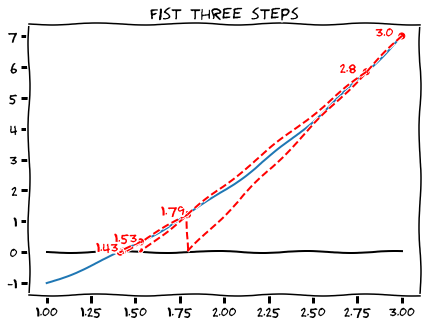
\includegraphics[width=0.6\linewidth]{images/secant.png}
\caption{Secant iterative method}\label{figure:SecantMethod}
\end{figure}
\end{example}

\begin{definition}\label{def:SecantMethod}\index{Secant method}\index{Secant method!iteration}\index{Secant method!recursive formula}
Given a function $f \colon \field{R} \to \field{R}$ and two initial guesses $x_0 \neq x_1$ satisfying $f(x_0) \neq f(x_1)$, we define the \emph{Secant method iteration} to be the sequence $\{ x_n \}_{n \in \field{N}}$ obtained by one of the following recursive formulas:
\begin{equation}\label{equation:SecantMethod}\index{Secant method!iteration}
\begin{split}
\bigg[\frac{f(x_n) - f(x_{n-1})}{x_n - x_{n-1}}\bigg] (x_{n+1} - x_n) = - f(x_n) \\
x_{n+1} = x_n - \bigg[ \frac{x_n - x_{n-1}}{f(x_n) - f(x_{n-1})} \bigg] f(x_n)
\end{split}
\end{equation}
The \emph{Secant method} refers to employing this sequence to search and approximate roots of the equation $f(x)=0$.
\end{definition}

\subsection{Efficiency of the Secant Method}
Let $f \colon \field{R} \to \field{R}$ be a real-valued function with a root $x^\star$, and let $\{ x_n \}_{n \in \field{N}}$ be a secant method iteration.  
\begin{align*}
x_{n+1} - x^\star &= x_n - \frac{x_n - x_{n-1}}{f(x_n) - f(x_{n-1})} f(x_n) - x^\star \\
&= (x_n - x^\star) \bigg( 1 - \frac{x_n - x_{n-1}}{f(x_n) - f(x_{n-1})}  \frac{f(x_n) - \overbrace{f(x^\star)}^0}{x_n - x^\star} \bigg) \\
&= (x_n - x^\star) \bigg(  1 - \frac{\Delta f [x_n, x^\star]}{\Delta f [x_{n-1}, x_n]} \bigg) \\
&= (x_n - x^\star) \frac{\Delta f [x_{n-1}, x_n] - \Delta f [x_n, x^\star]}{\Delta f [x_{n-1}, x_n]} \\
&= (x_n - x^\star) \frac{\Delta f [x_{n-1}, x_n] - \Delta f [x_n, x^\star]}{x_{n-1}-x^\star} \frac{x_{n-1}-x^\star}{\Delta f [x_{n-1}, x_n]} \\
&= (x_n - x^\star) (x_{n-1} - x^\star) \frac{\Delta f [x_{n-1}, x_n, x^\star]}{\Delta f [x_{n-1}, x_n]}
\end{align*}

We use this identity to prove the corresponding \emph{local convergence result}, as we did for the Newton-Raphson method:

\begin{theorem}[Local Convergence for the Secant Method]\label{theorem:LCScnt}\index{Secant method!Local convergence for}\index{Theorem!Local Convergence for Secant}
Let $x^\star$ be a simple root of the equation $f(x)=0$, and there exists $\varepsilon > 0$ so that 
\begin{itemize}
	\item $f$ is twice continuously differentiable in the interval $(x^\star-\varepsilon, x^\star + \varepsilon)$, and
	\item there are no critical points of $f$ on that interval.
\end{itemize}  
Set
\begin{equation*}
M(\varepsilon) = \max \bigg\{ \bigg\lvert \frac{f''(s)}{2f'(t)} \bigg\rvert : x^\star -\varepsilon < s,t < x^\star + \varepsilon \bigg\}.
\end{equation*}
If $\varepsilon$ is small enough so that $\varepsilon M(\varepsilon) < 1$, then
\begin{enumerate}
	\item \label{thm:LCScnt1} There are no other roots of $f$ in $(x^\star -\varepsilon, x^\star+\varepsilon)$.
	\item \label{thm:LCScnt2} Any Secant method iteration starting with initial guesses $x_0 \neq x_1$ (none of them equal to $x^\star$, and with $f(x_0) \neq f(x_1)$) in that interval will converge (quadratically) to $x^\star$
\end{enumerate} 
\end{theorem}

The proof is similar to the one for Theorem \ref{theorem:LCNR}, and is left as exercise.

\subsection{Generalization of the Secant Method to higher dimensions: Broyden's Method}
The objective now is the search of a root for a function $\boldsymbol{g} \colon \field{R}^d \to \field{R}^d$, which we assume of the form 
\begin{equation*}
\boldsymbol{g}(x_1, \dotsc, x_d) = \big[ g_1(x_1, \dotsc, x_d), \dotsc, g_d(x_1, \dotsc, x_d) \big]
\end{equation*}
for appropriate functions $g_k \colon \field{R}^d \to \field{R}$ ($1 \leq k \leq d$).  We start at an initial guess $\x_0 \in \field{R}^d$ and, if possible, we choose as $\x_1$ the first step of Newton-Raphson: 
\begin{equation*}
\transpose{\x_1} = \transpose{\x_0} - \big[ \gradient{\boldsymbol{g}}(\x_0) \big]^{-1} \cdot \transpose{\boldsymbol{g}(\x_0)}.
\end{equation*}
At that point we craft a linear approximation $\boldsymbol{L}_1 \colon \field{R}^d \to \field{R}^d$ to the graph of $\boldsymbol{g}$ that interpolates $\big( \x_0, \boldsymbol{g}(\x_0) \big)$ and $\big( \x_1, \boldsymbol{g}(\x_1) \big)$.  We may impose this \emph{secant property} by requesting $\boldsymbol{L}_1$ to be of the form\index{Secant property}
\begin{equation*}
\transpose{\boldsymbol{L}_1(\x)} = \transpose{\boldsymbol{g}(\x_1)} + \boldsymbol{A}_1 \cdot \transpose{(\x - \x_1)},
\end{equation*}
where $\boldsymbol{A}_1$ is a non-singular square matrix of size $d \times d$ that satisfies
\begin{equation*}
\boldsymbol{A}_1 \cdot \transpose{(\x_1 - \x_0)} = \transpose{\boldsymbol{g}(\x_1)} - \transpose{\boldsymbol{g}(\x_0)}.
\end{equation*}
At this point, we approximate the root of $\boldsymbol{g}$ by the root $\x_2$ of $\boldsymbol{L}_1$:
\begin{equation*}
\boldsymbol{A}_1 \cdot \transpose{(\x_2 - \x_1)} = -\transpose{\boldsymbol{g}(\x_1)},
\end{equation*}
or equivalently,
\begin{equation*}
\transpose{\x_2} = \transpose{\x_1} - \boldsymbol{A}_1^{-1} \cdot \transpose{\boldsymbol{g}(\x_1)}.
\end{equation*}
We repeat this process to obtain a sequence of approximations $\{ \x_n \}_{n \in \field{N}}$ via a sequence of non-singular square matrices $\boldsymbol{A}_n$ of size $d \times d$ that satisfy the secant property
\begin{equation}\label{equation:SecantProperty}
\boldsymbol{A}_n \cdot \transpose{(\x_{n+1} - \x_n)} = \transpose{\boldsymbol{g}(\x_{n+1})} - \transpose{\boldsymbol{g}(\x_n)}.
\end{equation}
The corresponding linear functions are given by 
\begin{equation*}
\transpose{\boldsymbol{L}_n (\x)} = \transpose{\boldsymbol{g}(\x_n)} + \boldsymbol{A}_n \cdot \transpose{(\x - \x_n)}.
\end{equation*}
The recurrence formula can then be expressed in any of the following two ways:
\begin{equation}
\begin{split}
\boldsymbol{A}_n \cdot \transpose{(\x_{n+1} - \x_n )} = -\transpose{\boldsymbol{g}(\x_n)}, \\
\transpose{\x_{n+1}} = \transpose{\x_n} - \boldsymbol{A}_n^{-1} \cdot \transpose{\boldsymbol{g}(\x_n)}
\end{split}
\end{equation}
We refer to this process as the \emph{Broyden Method} for finding roots.\index{Broyden method}

\begin{remark}
There is not a unique way to choose the matrices $\boldsymbol{A}_n$ in Broyden's method (and I encourage you to find one of your own devise).  A straightforward construction is given by the following recursive formulas:
\begin{gather}\index{Broyden method!recursive formula}\index{Broyden method!iteration}
\boldsymbol{A}_0 = \gradient{\boldsymbol{g}}(\x_0) \nonumber \\
\boldsymbol{A}_{n+1} = \boldsymbol{A}_n + \frac{\big[ \transpose{\big(\boldsymbol{g}(\x_{n+1})-\boldsymbol{g}(\x_n)\big)} - \boldsymbol{A}_n \transpose{(\x_{n+1}-\x_n)} \big] \otimes (\x_{n+1} -\x_n)}{\norm{\x_{n+1}-\x_n}^2} \label{equation:Broyden}
\end{gather}
\end{remark}

\begin{remark}
There are other possibilities for the selection of the point $\x_1$ that do not involve using the Jacobian $\gradient{\boldsymbol{g}}(\x_0)$ as the matrix $\boldsymbol{A}_0$.  For the purposes of root searching this choice is not too crucial but, as we shall see in the context of optimization, having the initial matrix $\boldsymbol{A}_0$ satisfy extra properties could be very advantageous.  To learn about different strategies in this regard, see e.g.~\cite[chapter 8]{dennis1996numerical}.
\end{remark}

\begin{example}\label{example:SecantPoly4}
Let's use this method to find any of the roots $(-1,-1)$, $(0,0)$, $(1,1)$ of the function $\boldsymbol{g}(x,y) = \big[ x^3-y, y^3 - x \big]$ from Example \ref{example:preNewton4poly4}.
Starting with initial guess $(x_0, y_0) = (-1, 1)$, we take the first step from Newton-Raphson:
\begin{align*}
\gradient{\boldsymbol{g}}(x_0, y_0) &= \begin{bmatrix} 3x_0^2 & -1 \\ -1 & 3y_0^2 \end{bmatrix} =  \begin{bmatrix} 3 & -1 \\ -1 & 3 \end{bmatrix} \\
\transpose{\boldsymbol{L}_0 (x, y)} &= \begin{bmatrix} -2 \\ 2 \end{bmatrix} + \begin{bmatrix} 3 & -1 \\ -1 & 3 \end{bmatrix} \cdot \begin{bmatrix} x \\ y \end{bmatrix} = \begin{bmatrix} 3x -y -2 \\ -x+3y +2 \end{bmatrix}
\end{align*}
This gives $(x_1, y_1) = (-1/2, 1/2)$ as root of $\boldsymbol{L}_0$.  For the second step, we compute the matrix $\boldsymbol{A}_1$ satisfying the secant property:
\begin{align*}
\boldsymbol{A}_1 &= \boldsymbol{A}_0 + \frac{\big[ \transpose{\big(\boldsymbol{g}(-1/2,1/2)-\boldsymbol{g}(-1,1)\big)} - \boldsymbol{A}_0 \transpose{[\tfrac{1}{2},-\tfrac{1}{2}]} \big] \otimes [\tfrac{1}{2},-\tfrac{1}{2}]}{\norm{[\tfrac{1}{2},-\tfrac{1}{2}]}^2} \\
&= \begin{bmatrix} 3 & -1 \\ -1 & 3 \end{bmatrix} + \frac{\bigg( \begin{bmatrix} -\tfrac{5}{8} -(-2) \\ \tfrac{5}{8}-2 \end{bmatrix} - \begin{bmatrix} 3 & -1 \\ -1 & 3 \end{bmatrix} \begin{bmatrix} \tfrac{1}{2} \\ -\tfrac{1}{2} \end{bmatrix} \bigg) \otimes \big[ \tfrac{1}{2}, -\tfrac{1}{2} \big]}{1/2} \\
&= \begin{bmatrix} 3 & -1 \\ -1 & 3 \end{bmatrix} + 2 \big( \big[ -\tfrac{5}{8}, \tfrac{5}{8} \big] \otimes \big[ \tfrac{1}{2}, -\tfrac{1}{2} \big] \big) \\
&= \begin{bmatrix} 3 & -1 \\ -1 & 3 \end{bmatrix} + 2 \begin{bmatrix} -\tfrac{5}{8} \cdot \tfrac{1}{2} & -\tfrac{5}{8}\cdot \big( -\tfrac{1}{2} \big) \\ \tfrac{5}{8} \cdot \tfrac{1}{2} & \tfrac{5}{8} \cdot \big(- \tfrac{1}{2} \big) \end{bmatrix} \\
&= \begin{bmatrix} 3 & -1 \\ -1 & 3 \end{bmatrix} + \begin{bmatrix} -5/8 & 5/8 \\ 5/8 & -5/8 \end{bmatrix} = \begin{bmatrix} 19/8 & -3/8 \\ -3/8 & 19/8 \end{bmatrix}
\end{align*}
This gives a linear approximation 
\begin{equation*}
\transpose{\boldsymbol{L}_1(x,y)} = \begin{bmatrix} -5/8 \\ 5/8 \end{bmatrix} + \begin{bmatrix} 19/8 & -3/8 \\ -3/8 & 19/8 \end{bmatrix} \cdot \begin{bmatrix} x + 1/2 \\ y - 1/2 \end{bmatrix} = \begin{bmatrix} \tfrac{19}{8}x-\tfrac{3}{8}x + \tfrac{3}{4} \\ \\ -\tfrac{3}{8}x+\tfrac{19}{8}y - \tfrac{3}{4} \end{bmatrix}
\end{equation*}
which has root $(x_2, y_2) = (-3/11, 3/11)$.

If we continue the computations, we arrive to the root $(0,0)$ to an accuracy of 6 decimal places in just 5 steps!
\begin{center}
\begin{tabular}{|r|r|r|r@{, }l|} \hline 
$n$ & $x_n$ & $y_n$ & $f(x_n$ & $y_n)$ \\ \hline \hline 
$1$ & $-1.000000$ & $1.000000$ & $\big(-2.000000$ & $2.000000 \big)$ \\ \hline 
$2$ & $-0.500000$ & $0.500000$ & $\big(-0.625000$ & $0.625000 \big)$ \\ \hline 
$2$ & $-0.272727$ & $0.272727$ & $\big(-0.293013$ & $0.293013 \big)$ \\ \hline 
$3$ & $-0.072136$ & $0.072136$ & $\big(-0.072511$ & $0.072511 \big)$ \\ \hline 
$4$ & $-0.006172$ & $0.006172$ & $\big(-0.006172$ & $0.006172 \big)$ \\ \hline 
$5$ & $-0.000035$ & $0.000035$ & $\big(-0.000035$ & $0.000035 \big)$ \\ \hline 
$6$ & $-0.000000$ & $0.000000$ & $\big(-0.000000$ & $0.000000 \big)$ \\ \hline 
\end{tabular}
\end{center}
\end{example}

\subsection{Secant Methods for Optimization}

Given a real-valued function $f \colon \field{R}^d \to \field{R}$, we may apply Broyden's method to search for roots of the gradient $\gradient{f} \colon \field{R}^d \to \field{R}^d$.  As it happened with Newton's method, we are not guaranteed convergence to a local minimum.

\begin{example}
As we did in Example \ref{example:NewtonPoly4}, we may explore the convergence to different critical points of the polynomial $p_4(x,y) = x^4-4xy+y^4$ using different initial guesses.  Note once again that the gradient of $p_4$ is the function $\gradient{p_4} = \boldsymbol{g}$ from Example \ref{example:SecantPoly4}:

For instance, starting with $(x_0,y_0) = (-1,1)$ we converge to the critical point $(0,0)$, which is not a local minimum.
\end{example}

\section{The Method of Steepest Descent}\index{Steepest descent}\index{Gradient!descent|see {Steepest descent}}

The method of \emph{Steepest Descent} (also known as the method of \emph{Gradient Descent}) is based upon the following property of gradients that we learned in Vector Calculus:

\begin{theorem}
If $f \colon \field{R}^d \to \field{R}$ is continuously differentiable, then at any point $\x \in \field{R}^d$, the vector $-\gradient{f}(\x)$ points in the direction of most rapid decrease for $f$ at $\x$.  The rate of decrease of $f$ at $\x$ in this direction is precisely $-\norm{\gradient{f}(\x)}$.
\end{theorem}

\begin{remark}\index{Steepest descent!direction of}\index{Direction!of steepest descent}
For this reason, the vector $-\gradient{f}(\x)/\norm{\gradient{f}(\x)}$ is called the \emph{direction of steepest descent} of $f$ at $\x$.
\end{remark}

\separator

In order to search for a local minimum for a twice continuously differentiable function $f\colon \field{R}^d \to \field{R}$, we start by choosing an initial guess $\x_0$.  
\begin{enumerate}
	\item Restrict the function $f$ over the line through $\x_0$ in the direction of $-\gradient{f}(\x_0)$:
	\begin{equation*}
	\varphi_0(t) = f\big( \x_0 - t \gradient{f}(\x_0) \big), \quad t\geq 0
	\end{equation*}
	\item \emph{Line-search}: Search for the value of $t_0 \geq 0$ that minimizes $\varphi_0$, and set\index{Line-search}
	\begin{equation*}
	\x_1 = \x_0 - t_0\gradient{f}(\x_0)
	\end{equation*}
	\item Repeat this process to get the sequence
	\begin{gather}\label{equation:SteepestDescent}
	\begin{split}
	&\x_{n+1} = \x_n - t_n \gradient{f}(\x_n), \\ &t_n = \argmin_{t\geq 0} \varphi_n(t) = \argmin_{t\geq 0} f\big(\x_n - t\gradient{f}(\x_n)\big)
	\end{split}
	\end{gather}
\end{enumerate}

\begin{remark}\index{Steepest descent!sequence of}
Sequences constructed following the formula in \eqref{equation:SteepestDescent} are said to be \emph{sequences of Steepest Descent} for $f$.

Unlike Newton-Raphson or the secant methods, this algorithm guarantees that these sequences are non-increasing: $f(\x_{n+1}) \leq f(\x_n)$ for all $n \in \field{N}$.  And even better: if there is convergence, their limit must be a critical point of $f$.  These results are formalized in Theorems \ref{theorem:SteepestDescentDescends} and \ref{theorem:SteepestDescentConvergesToCritical}  below.

Steepest descent sequences have another interesting property: on each step $n$, the direction of steepest descent is perpendicular to the direction of steepest descent of step $n+1$ (!!)  We state and prove this result in Theorem \ref{theorem:SteepestDescentPerpSteps}.
\end{remark}

\begin{theorem}\label{theorem:SteepestDescentDescends}
Let $f\colon \field{R}^d \to \field{R}$ be a continuously differentiable real-valued function, and let $\{ \x_n \}_{n\in\field{N}}$ be a sequence of steepest descent for $f$.  If $\gradient{f}(\x_N) \neq 0$, then $f(\x_{N+1}) < f(\x_N)$.
\end{theorem}

\begin{theorem}\label{theorem:SteepestDescentConvergesToCritical}
Let $f\colon \field{R}^d \to \field{R}$ be a real-valued function, let $\x_0 \in \field{R}^d$ be an initial guess.  Assume $S = \{ \x \in \field{R}^d :  f(\x) \leq f(\x_0) \}$ is a compact set and $f$ is continuously differentiable in $S$.  Under these conditions, the limit of any convergent subsequence of the associated sequence of steepest descent $\{ \x_n \}_{n\in \field{N}}$ is a critical point of $f$.
\end{theorem}

\begin{theorem}\label{theorem:SteepestDescentPerpSteps}
Let $f \colon \field{R}^d \to \field{R}$ be a continuously differentiable real-valued function, and $\{ \x_n \}_{n\in\field{N}}$ a sequence of steepest descent for $f$.  For any $n \in \field{N}$, $\langle \x_{n+2} - \x_{n+1}, \x_{n+1} - \x_n \rangle = 0$.
\end{theorem}
\begin{proof}
Consider for each $n \in \field{N}$ the function $\varphi_n(t) = f\big(\x_n -t \gradient{f}(\x_x)\big)$, with a global minimum at $t_n \geq 0$.  It must then be
\begin{equation*}
0 = \varphi_n'(t_n) = \langle \gradient{f}(\x_n), -\gradient{f}\big( \x_n - t_n \gradient{f}(\x_n)\big) \rangle = - \langle \gradient{f}(\x_{n+1}), \gradient{f}(\x_n) \rangle,
\end{equation*}
which proves that the gradient of consecutive terms of the sequence of steepest descent for $f$ are perpendicular.  Now, by virtue of the recurrence formula \eqref{equation:SteepestDescent},
\begin{align*}
\langle \x_{n+2} - \x_{n+1}, &\,\x_{n+1} - \x_n \rangle = \langle t_{n+1}\gradient{f}(\x_{n+1}), t_n \gradient{f}(\x_n) \rangle \\
&= t_{n+1}t_n \langle \gradient{f}(\x_{n+1}), \gradient{f}(\x_n) \rangle = 0, 
\end{align*}
which proves the statement.
\end{proof}

\begin{example}
For the polynomial function $p_4(x,y) = x^4-4xy+y^4$ from Example \ref{example:NewtonPoly4}, using the same initial guesses as in Example \ref{example:preNewton4poly4}, we find the following behavior:
\begin{itemize}
	\item Starting at $(x_0, y_0) = (-1.0,1.0)$, the sequence jumps to $(0,0)$ in one step.  At that point, since the gradient of the function is zero, the method of Steepest descent ceases to work.
	% \begin{table}[ht!]
	\begin{center}
	\begin{tabular}{|r|r|r|r|} \hline 
	$n$ & $x_n$ & $y_n$ & $f(x_n,y_n)$ \\ \hline \hline 
	$0$ & $-1.000000$ & $1.000000$ & $6.000000$ \\ \hline 
	$1$ & $0.000000$ & $0.000000$ & $0.000000$ \\ \hline 
	$2$ & \texttt{nan} & \texttt{nan} & \texttt{nan} \\ \hline 
	\end{tabular}
	% \caption{Steepest Descent: Convergence to $(0,0)$ accurately in exactly one step.}
	% \label{table:SD00}
	% \end{table}
	\end{center}
	\item Starting at $(x_0,y_0) = (3.5, 2.1)$, the sequence converges to $(1,1)$.
	% \begin{table}[ht!]
	\begin{center}
	\begin{tabular}{|r|r|r|r|} \hline 
	$n$ & $x_n$ & $y_n$ & $f(x_n,y_n)$ \\ \hline \hline 
	$0$ & $3.500000$ & $2.100000$ & $140.110600$ \\ \hline 
	$1$ & $1.044472$ & $1.753064$ & $3.310777$ \\ \hline 
	$2$ & $1.141931$ & $1.063276$ & $-1.878163$ \\ \hline 
	$3$ & $1.008581$ & $1.044435$ & $-1.988879$ \\ \hline 
	$4$ & $1.013966$ & $1.006319$ & $-1.998931$ \\ \hline 
	$5$ & $1.000898$ & $1.004472$ & $-1.999891$ \\ \hline 
	$6$ & $1.001437$ & $1.000651$ & $-1.999989$ \\ \hline 
	$7$ & $1.000093$ & $1.000461$ & $-1.999999$ \\ \hline 
	% \end{tabular}~\begin{tabular}{|r|r|r|r|} \hline 
	% $n$ & $x_n$ & $y_n$ & $f(x_n,y_n)$ \\ \hline \hline 
	$8$ & $1.000149$ & $1.000067$ & $-2.000000$ \\ \hline 
	$9$ & $1.000010$ & $1.000048$ & $-2.000000$ \\ \hline 
	$10$ & $1.000015$ & $1.000007$ & $-2.000000$ \\ \hline 
	$11$ & $1.000001$ & $1.000005$ & $-2.000000$ \\ \hline 
	$12$ & $1.000002$ & $1.000001$ & $-2.000000$ \\ \hline 
	$13$ & $1.000000$ & $1.000001$ & $-2.000000$ \\ \hline 
	$14$ & $1.000000$ & $1.000000$ & $-2.000000$ \\ \hline 
	$15$ & $1.000000$ & $1.000000$ & $-2.000000$ \\ \hline 
	\end{tabular}
	% \caption{Steepest Descent: Convergence to $(1,1)$ with 6-digit accuracy in 13 steps.}
	% \label{table:SD11}
	% \end{table}
	\end{center}
	\item Starting at $(x_0, y_0) = (-13.5, -7.3)$, the sequence converges to $(1,1)$ as well.
	% \begin{table}[ht!]
	\begin{center}
	\begin{tabular}{|r|r|r|r|} \hline 
	$n$ & $x_n$ & $y_n$ & $f(x_n,y_n)$ \\ \hline \hline 
	$0$ & $-13.500000$ & $-7.300000$ & $35660.686600$ \\ \hline 
	$1$ & $2.362722$ & $-4.871733$ & $640.498302$ \\ \hline 
	$2$ & $1.434154$ & $1.194162$ & $-0.586492$ \\ \hline 
	$3$ & $1.021502$ & $1.130993$ & $-1.896212$ \\ \hline 
	$4$ & $1.038817$ & $1.017881$ & $-1.991558$ \\ \hline 
	$5$ & $1.002305$ & $1.012291$ & $-1.999167$ \\ \hline 
	$6$ & $1.003909$ & $1.001808$ & $-1.999917$ \\ \hline 
	$7$ & $1.000236$ & $1.001246$ & $-1.999992$ \\ \hline 
	% \end{tabular}~\begin{tabular}{|r|r|r|r|} \hline 
	% $n$ & $x_n$ & $y_n$ & $f(x_n,y_n)$ \\ \hline \hline 
	$8$ & $1.000399$ & $1.000185$ & $-1.999999$ \\ \hline 
	$9$ & $1.000024$ & $1.000127$ & $-2.000000$ \\ \hline 
	$10$ & $1.000041$ & $1.000019$ & $-2.000000$ \\ \hline 
	$11$ & $1.000002$ & $1.000013$ & $-2.000000$ \\ \hline 
	$12$ & $1.000004$ & $1.000002$ & $-2.000000$ \\ \hline 
	$13$ & $1.000000$ & $1.000001$ & $-2.000000$ \\ \hline 
	$14$ & $1.000000$ & $1.000000$ & $-2.000000$ \\ \hline 
	$15$ & $1.000000$ & $1.000000$ & $-2.000000$ \\ \hline 
	\end{tabular}
	% \caption{Steepest Descent: Convergence to $(1,1)$ with 6-digit accuracy in 14 steps.}
	% \label{table:SD-1-1}
	% \end{table}
	\end{center}
\end{itemize}
\begin{figure}[ht!]
% \begin{tabular}{c}
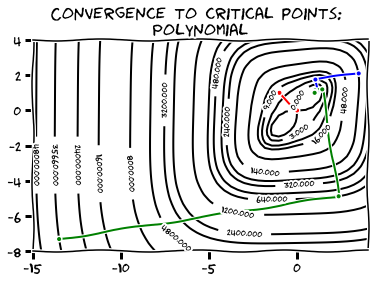
\includegraphics[width=0.7\linewidth]{images/convergenceSteepest.png}
% 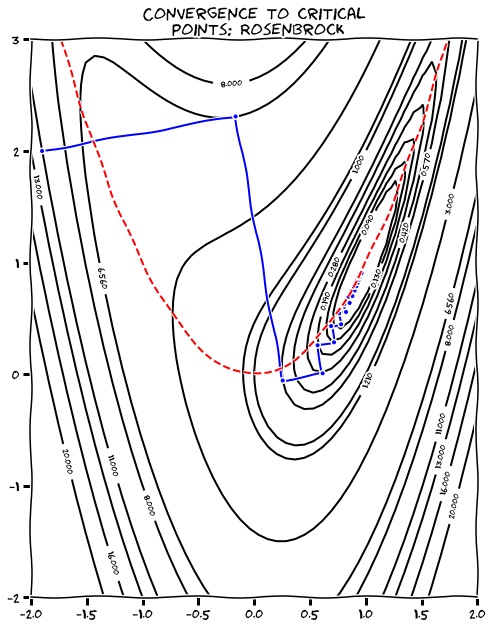
\includegraphics[width=0.65\linewidth]{images/SDR3.png}
% \end{tabular}
\caption{The Method of Steepest Descent: Polynomial function}
\label{figure:SteepestConvergenceP}
\end{figure}
\end{example}

\begin{example}\label{example:SDR}\index{Function!Rosenbrock}
Notice what happens when we try to implement the same process on the Rosenbrock function $\mathcal{R}_{1,1}(x,y) = (1-x)^2 + (y-x^2)^2$, with the initial guess $(x_0, y_0) = (-2,2)$.  The sequence does converge to the minimum $(1,1)$, albeit very slowly.
\begin{center}
\begin{tabular}{|r|r|r|r|} \hline 
 $n$ & $x_n$ & $y_n$ & $f(x_n,y_n)$ \\ \hline \hline 
$0$ & $-2.000000$ & $2.000000$ & $13.000000$ \\ \hline 
$1$ & $-0.166290$ & $2.309522$ & $6.567163$ \\ \hline 
$2$ & $0.256054$ & $-0.056128$ & $0.568264$ \\ \hline 
$3$ & $0.613477$ & $0.007683$ & $0.285318$ \\ \hline 
$4$ & $0.568566$ & $0.259241$ & $0.190235$ \\ \hline 
$5$ & $0.715784$ & $0.285524$ & $0.132227$ \\ \hline 
$6$ & $0.689755$ & $0.431319$ & $0.098227$ \\ \hline 
$7$ & $0.779264$ & $0.447299$ & $0.074310$ \\ \hline 
$8$ & $0.761554$ & $0.546496$ & $0.057977$ \\ \hline 
$9$ & $0.823325$ & $0.557524$ & $0.045696$ \\ \hline 
$10$ & $0.810322$ & $0.630358$ & $0.036667$ \\ \hline 
$11$ & $0.855862$ & $0.638488$ & $0.029614$ \\ \hline 
$12$ & $0.845883$ & $0.694385$ & $0.024199$ \\ \hline 
$13$ & $0.880846$ & $0.700627$ & $0.019862$ \\ \hline 
$14$ & $0.872964$ & $0.744776$ & $0.016437$ \\ \hline 
$15$ & $0.900551$ & $0.749702$ & $0.013647$ \\ \hline 
$16$ & $0.894200$ & $0.785276$ & $0.011399$ \\ \hline 
\end{tabular}~\begin{tabular}{|r|r|r|r|} \hline
 $n$ & $x_n$ & $y_n$ & $f(x_n,y_n)$ \\ \hline \hline 
$17$ & $0.916394$ & $0.789239$ & $0.009544$ \\ \hline 
$18$ & $0.911201$ & $0.818326$ & $0.008028$ \\ \hline 
$19$ & $0.929317$ & $0.821560$ & $0.006766$ \\ \hline 
$20$ & $0.925024$ & $0.845608$ & $0.005723$ \\ \hline 
$21$ & $0.939976$ & $0.848277$ & $0.004847$ \\ \hline 
$22$ & $0.936397$ & $0.868329$ & $0.004118$ \\ \hline 
$23$ & $0.948845$ & $0.870551$ & $0.003502$ \\ \hline 
$24$ & $0.945840$ & $0.887385$ & $0.002986$ \\ \hline 
$25$ & $0.956276$ & $0.889248$ & $0.002548$ \\ \hline 
$26$ & $0.953739$ & $0.903457$ & $0.002178$ \\ \hline 
$27$ & $0.962537$ & $0.905028$ & $0.001864$ \\ \hline 
$28$ & $0.960386$ & $0.917075$ & $0.001597$ \\ \hline 
$29$ & $0.967837$ & $0.918405$ & $0.001369$ \\ \hline 
$30$ & $0.966007$ & $0.928657$ & $0.001176$ \\ \hline 
$31$ & $0.972342$ & $0.929788$ & $0.001010$ \\ \hline 
$32$ & $0.970780$ & $0.938539$ & $0.000869$ \\ \hline 
$33$ & $0.976182$ & $0.939503$ & $0.000748$ \\ \hline 
\end{tabular}
\end{center}
\end{example}

\begin{figure}[ht!]
% \begin{tabular}{c}
% 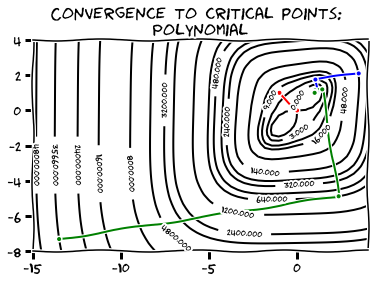
\includegraphics[width=0.65\linewidth]{images/convergenceSteepest.png} \\
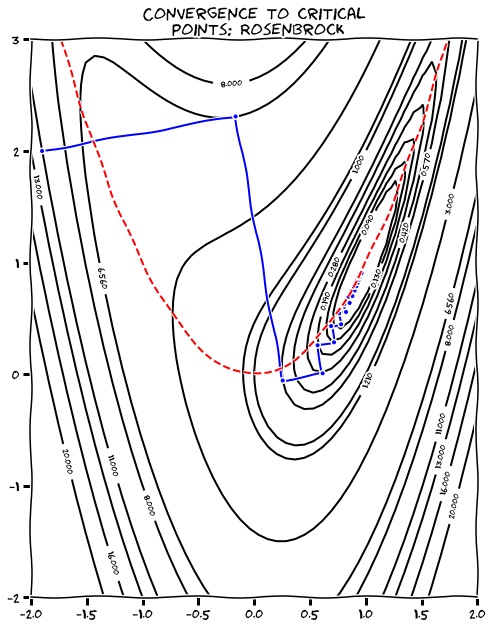
\includegraphics[width=0.6\linewidth]{images/SDR3.png}
% \end{tabular}
\caption{The Method of Steepest Descent: Rosenbrock Function}
\label{figure:SteepestConvergenceR}
\end{figure}

\subsection{Efficiency of Steepest Descent Method}

The analysis of efficiency of the method of Steepest descent is quite involved, but it boils down to studying the efficiency of Steepest descent for quadratic functions---since any function can be approximated using a Taylor's polynomial of degree two.  We will study that easier case in these notes.

\begin{theorem}[Taylor's Formula]\index{Theorem!Taylor's formula}
If $f\colon \field{R}^d \to \field{R}$ is a real-valued function of $d$ variables with continuous first and second partial derivatives on $\field{R}^d$, then for any choice $\x, \y \in \field{R}^d$, there exists a point $\boldsymbol{\xi} = \boldsymbol{\xi}(\x, \y)$ in the segment joining $\x$ and $\y$ so that
\begin{equation*}
f(\x) = f(\y) + \langle \gradient{f}(\y), \x - \y \rangle + \tfrac{1}{2} \quadratic{\Hess{f}(\boldsymbol{\xi})}(\x - \y)
\end{equation*}
\end{theorem}

\separator

Assume we have a quadratic function $p\colon \field{R}^d \to \field{R}$ satisfying $p(\boldsymbol{0}) = 0$.  There exist a $d$-dimensional vector $D = \big[q_1, \dotsc, q_d\big]$ and a symmetric matrix $Q = \big[ q_{jk} \big]_{j,k=1}^d$ (with $q_{jk}=q_{kj}$ for all $1\leq j,k \leq d$) so that
\begin{equation*}
p(\x) = \langle D, \x \rangle + \tfrac{1}{2}\quadratic{Q}(\x) = \sum_{k=1}^d \big( \tfrac{1}{2}q_{kk}x_k^2 + q_k x_k\big) + \sum_{1\leq j<k \leq d} q_{jk} x_j x_k
\end{equation*}
The gradient of this function is thus $\gradient{p}(\x) = x \cdot Q + D$.  It has one unique critical point $\xstar = -D Q^{-1}$ (Why?).  At that point, it is 
\begin{align}
p(\xstar) &= \tfrac{1}{2} \big( -D Q^{-1} \big)  Q \transpose{\big( -D Q^{-1} \big)} + D \transpose{\big( -D Q^{-1} \big)} \nonumber \\ 
&= \tfrac{1}{2} D Q^{-1} \transpose{D} - D Q^{-1} \transpose{D} \nonumber \\
&= -\tfrac{1}{2} D Q^{-1} \transpose{D} = -\tfrac{1}{2}\quadratic{(Q^{-1})}(D). \label{equation:pstarSD}
\end{align}
If $\x_n$ is a term in a sequence of steepest descent, then to compute $\x_{n+1}$ we proceed as follows:
\begin{enumerate}
	\item The direction of steepest descent at $\x_n$ is 
	\begin{equation*}\v_n = -\gradient{p}(\x_n) = -(x_n Q + D).
	\end{equation*}
	\item The restriction $\varphi\colon (0,\infty) \to \field{R}$ of the quadratic function $p$ over the half-line through $\x_n$ in the direction $\v_n$ is given by
	\begin{align*}
	\varphi(t) &= p( \x_n + t \v_n ) \\
	&= \tfrac{1}{2}(\x_n + t\v_n ) Q \transpose{(\x_n + t\v_n )} + D\transpose{(\x_n + t\v_n )} \\
	&= \tfrac{1}{2} \x_n Q \transpose{(\x_n + t\v_n )} + \tfrac{1}{2}t\v_n Q \transpose{(\x_n + t\v_n )} \\
	&\quad+D \transpose{\x}_n + tD \transpose{\v}_n \\
	&= \tfrac{1}{2}\x_n Q \transpose{\x}_n + \tfrac{1}{2} t\x_n Q \transpose{\v}_n + \tfrac{1}{2} t \v_n Q \transpose{\x}_n + \tfrac{1}{2} t^2 \v_n Q \transpose{\v}_n \\
	&\quad + D \transpose{\x}_n + t D \transpose{\v}_n \\
	&= \tfrac{1}{2} \underbrace{\v_n Q \transpose{\v}_n}_{\quadratic{Q}(\v_n)} t^2 + \underbrace{\tfrac{1}{2}\x_n Q \transpose{\x}_n + D \transpose{\x}_n}_{p(\x_n)} + tD\transpose{\v}_n + t \x_n Q \transpose{\v}_n \\
	&= \tfrac{1}{2} \quadratic{Q}(\v_n) t^2  + p(\x_n) + t \underbrace{\big( x_n Q + D \big)}_{-\v_n} \transpose{\v}_n \\
	&= \tfrac{1}{2}t^2 \v_n Q \transpose{\v}_n -  t \v_n \transpose{\v}_n + p(\x_n) \\
	&= \tfrac{1}{2} \quadratic{Q}(\v_n)t^2 - \norm{\v_n}^2 t + p(\x_n)
	\end{align*}
	\item The restriction function has its global minimum at
	\begin{equation*}
	t_n = \frac{\norm{\v_n}^2}{\quadratic{Q}(\v_n)};
	\end{equation*}
	therefore, the next iteration occurs at
	\begin{equation*}
	x_{n+1} = x_n + t_n \v_n = x_n + \frac{\norm{\v_n}^2}{\quadratic{Q}(\v_n)} \v_n 
	\end{equation*}
\end{enumerate}

\separator

We want to observe the convergence behavior of the sequence of evaluations $\{ p(\x_n) \}_{n \in \field{N}}$ to $p(\xstar)$.  We have
\begin{align*}
p(\x_{n+1}) &= p(\x_n + \tfrac{\norm{\v_n}^2}{\quadratic{Q}(\v_n)} \v_n) \\
&= \tfrac{1}{2} \quadratic{Q}(\v_n) \big( \tfrac{\norm{\v_n}^2}{\quadratic{Q}(\v_n)} \big)^2 - \norm{\v_n}^2 \tfrac{\norm{\v_n}^2}{\quadratic{Q}(\v_n)} + p(\x_n) \\
&= p(\x_n) - \frac{\norm{\v_n}^4}{2\quadratic{Q}(\v_n)}; 
\intertext{therefore,}
\frac{p(\x_{n+1}) - p(\xstar)}{p(\x_n)- p(\xstar)} &= \frac{p(\x_n) - p(\xstar) - \frac{\norm{\v_n}^4}{2\quadratic{Q}(\v_n)}}{p(\x_n) - p(\xstar)} \\
&= 1 - \frac{\norm{\v_n}^4}{ 2\quadratic{Q}(\v_n) \big( p(\x_n) - p(\xstar) \big)} \\
&= 1 - \frac{\norm{\v_n}^4}{2\quadratic{Q}(\v_n) \big( \tfrac{1}{2}\x_n Q \transpose{\x}_n + D \transpose{\x}_n + \tfrac{1}{2} DQ^{-1}\transpose{D} \big)} \\
&= 1 - \frac{\norm{\v_n}^4}{ \quadratic{Q}(\v_n) \big( \x_n Q \transpose{\x}_n+ 2D\transpose{\x}_n + DQ^{-1}\transpose{D} \big) }.
\end{align*}
Note in the denominator we may rewrite some of the terms:
\begin{align*}
\x_n Q \transpose{\x}_n &= \x_n Q (Q^{-1}Q) \transpose{\x}_n = (\x_n Q) Q^{-1} \transpose{(\x_n Q)}, \\
2D \transpose{\x}_n &= D\transpose{\x}_n + D\transpose{\x}_n = \x_n \transpose{D} + D (Q^{-1}Q) \transpose{\x}_n \\
&= \x_n (QQ^{-1}) \transpose{D} + D Q^{-1} \transpose{(\x_n Q)} \\
&= (\x_n Q) Q^{-1} \transpose{D} + D Q^{-1} \transpose{(\x_n Q)}.
\end{align*} 
This allows us to rewrite in the following convenient form 
\begin{align*}
\frac{p(\x_{n+1}) - p(\xstar)}{p(\x_n)- p(\xstar)} &= 1 - \frac{\norm{\v_n}^4}{ \quadratic{Q}(\v_n) (\x_n Q + D) Q^{-1} \transpose{(\x_nQ + D)} } \\
&= 1 - \frac{\norm{\v_n}^4}{\quadratic{Q}(\v_n) \quadratic{(Q^{-1})}(\v_n)}.
\end{align*}

We are ready to state the main result of this subsection:
\begin{theorem}\label{theorem:KantorovichEstimate}\index{Steepest descent!error}
Given a $d$-dimensional vector $D$, and a positive definite symmetric matrix $Q$ of size $d \times d$, consider the quadratic function $p(\x) = \tfrac{1}{2}\quadratic{Q}(\x) + \langle D , \x \rangle$.  Any sequence $\{ \x_n \}_{n \in \field{N}}$ of steepest descent converges to the global minimum $\xstar = -DQ^{-1}$.  The sequence of evaluations $\{ p(\x_n) \}_{n \in \field{N}}$ converges linearly to $p(\xstar) = -\tfrac{1}{2}\quadratic{(Q^{-1})}(D)$.  In particular, if $0 < \lambda_1 \leq \lambda_2 \leq \dotsb \leq \lambda_d$ are the eigenvalues of $Q$, then 
\begin{equation*}
\frac{p(\x_{n+1}) - p(\xstar)}{p(\x_n)- p(\xstar)} \leq \bigg( \frac{\lambda_d -\lambda_1}{\lambda_d + \lambda_1} \bigg)^2
\end{equation*}
\end{theorem}
\begin{proof}
We start by offering the following lower bound estimate\footnote{This is left as and advanced exercise. It is not too tricky; if you are stuck, see e.g.~\cite[section 1.3.1]{bertsekas1999nonlinear} for a proof.} involving the associated directions of steepest descent $\v_n$ in terms of the largest and smallest eigenvalues of $Q$.  For all $n \in \field{N}$,
\begin{equation}\label{equation:KantorovichEstimate}\index{Theorem!Kantorovich estimate}
\frac{\norm{\v_n}^4}{\quadratic{Q}(\v_n) \quadratic{(Q^{-1})}(\v_n)} \geq \frac{4\lambda_0\lambda_d}{(\lambda_0 + \lambda_d)^2}
\end{equation}
We have then
\begin{align*}
\frac{p(\x_{n+1}) - p(\xstar)}{p(\x_n)- p(\xstar)} &= 1 - \frac{\norm{\v_n}^4}{ \quadratic{Q}(\v_n) \quadratic{(Q^{-1})}(\v_n) } \\
&\leq 1 - \frac{4\lambda_1 \lambda_d}{(\lambda_1 + \lambda_d)^2} = \bigg( \frac{\lambda_d - \lambda_1}{\lambda_d + \lambda_1} \bigg)^2 \qedhere
\end{align*}
\end{proof}

\begin{example}\label{example:SDconvergenceRate}
The global minimum value of the quadratic function $p(x,y) = 5x^2 + 5y^2 -xy -11x +11y +11$ is zero, and found at $(1,-1)$.  Notice that we may write this function in the form $p(x,y) = \tfrac{1}{2}\quadratic{Q}(x,y) + \langle D, [x,y] \rangle + 11$, where
\begin{equation*}
D = [ -11, 11], \qquad Q = \begin{bmatrix} 10 & -1 \\ 10 & -1 \end{bmatrix}.
\end{equation*}
The symmetric matrix $Q$ has eigenvalues $\lambda_1 = 9 >0$, $\lambda_2 = 11 > 0$ and is therefore positive definite.  Theorem \ref{theorem:KantorovichEstimate} states that sequences of steepest descent exhibit linear convergence with a rate of convergence not larger than $\delta = \big( \tfrac{11-9}{11+9} \big)^2 = 0.01$.

Observe the computations of the first six iterations for values of the ratios $\frac{p(\x_n)}{p(\x_{n-1})}$ when we use $(1.5,3.5)$ as our initial guess.
\begin{center}
\begin{tabular}{|r|r|r|r|r|} \hline 
 $n$ & $x_n$ & $y_n$ & $p(x_n,y_n)$ & $\boldsymbol{\frac{p(x_n,y_n)}{p(x_{n-1},y_{n-1})}}$ \\ \hline \hline 
$0$ & $1.5000000000$ & $3.5000000000$ & $100.2500000000$ &  \\ \hline 
$1$ & $1.4498874016$ & $-0.9600212545$ & $1.0019989373$ & $\boldsymbol{0.0099950019}$ \\ \hline 
$2$ & $1.0049975009$ & $-0.9550224916$ & $0.0100149812$ & $\boldsymbol{0.0099950019}$ \\ \hline 
$3$ & $1.0044966254$ & $-0.9996004124$ & $0.0001000998$ & $\boldsymbol{0.0099950019}$ \\ \hline 
$4$ & $1.0000499500$ & $-0.9995504497$ & $0.0000010005$ & $\boldsymbol{0.0099950019}$ \\ \hline 
$5$ & $1.0000449438$ & $-0.9999960061$ & $0.0000000100$ & $\boldsymbol{0.0099950042}$ \\ \hline 
$6$ & $1.0000004993$ & $-0.9999955067$ & $0.0000000001$ & $\boldsymbol{0.0099950528}$ \\ \hline 
\end{tabular}
\end{center}
\end{example}

\section{Effective Algorithms for Unconstrained Optimization}
All of the methods we have explored so far (Newton-Raphson, Secant methods, Steepest descent) offer sound algorithms to compute local extrema of real-valued functions $f \colon \field{R}^d \to \field{R}$. They do have some pros and cons.  
\begin{itemize}
	\item The method of Steepest descent produces non-increasing iterations.
	\item In order to obtain new approximations on each Steepest descent iteration, we have to solve many different one-dimensional optimizations, each of them offering their own computational issues. 
	\item Both Newton-Raphson and Secant methods offers faster sequences, but we cannot always guarantee convergence.  
	\item Another drawback of Newton-Raphson is the fact that we do need to evaluate the function itself, its gradient and Hessian matrix. 
	\item The recurrence formulas of Broyden's method are simple, and require only evaluations of the function itself.
\end{itemize}

The goal of this section is precisely gathering the best properties of the previous methods, so we may craft new methods with all the advantages, but none of the shortcomings.  

\separator

Given a function $f \colon \field{R}^d \to \field{R}$ with continuous first partial derivatives, and a given initial guess $\x_0 \in \field{R}^d$, we search for a recursive formula to approximate a minimum of $f$.  We request that this formula has the form
\begin{equation*}
\x_{n-1} = \x_n + t_n \w_n,
\end{equation*}
with positive parameters $t_n > 0$, and vectors $\w_n$ satisfying the following criteria:
\begin{description}
	\item[Non-increasing sequences] $f(\x_{n+1}) < f(\x_n)$ whenever $\gradient{f}(\x_n) \neq 0$. 

	\noindent This is achieved by requiring the vectors $\omega_n$ to have an angle larger than $\pi/2$ with respect to $\gradient{f}(\x_n)$:
	\begin{equation}
	\langle \w_n , \gradient{f}(\x_n) \rangle < 0.\label{Criterion2}
	\end{equation}
	Why does this work? Consider at each step $n \in \field{N}$ the restriction $\varphi_n(t)=f\big( \x_n + t \w_n \big)$ of $f$ over the line $\x_n + t \w_n$ with $t>0$.  We have then $\varphi_n'(0) = \langle \gradient{f}(\x_n), \w_n \rangle < 0$ (a decreasing function near $t=0$).  We have a guaranteed value $t_n > 0$ (that could be very small) that give us a point $\x_{n+1} = \x_n + t_n \w_n$ with $f(\x_{n+1}) < f(\x_n)$.
	\item[Control over length of steps] The steps $t_n$ are not \emph{too short, nor too long}.

	\noindent This is achieved by picking first $0 < \mu < \lambda < 1$ and forcing vectors $\omega_n$ that satisfy
	\begin{gather}
	\langle \w_n , \gradient{f}(\x_{n+1}) - \lambda \gradient{f} (\x_n) \rangle > 0 \label{Criterion3}\\
	f(\x_{n+1}) \leq f(\x_n) + \mu t_n \langle \w_n \gradient{f}(\x_n) \rangle \label{Criterion4}
	\end{gather}
	if this is at all possible.
	\item[Easy to compute] Duh!
\end{description}

\separator

Is it possible to create a iteration satisfying these criteria?  The following result gives us a condition that helps in this regard:

\begin{theorem}[Wolfe]\label{theorem:Wolfe}\index{Theorem!Wolfe}
Suppose that $f \colon \field{R}^d \to \field{R}$ is a real-valued function with continuous partial derivatives.  Assume there exists $M \in \field{R}$ so that $f(x) \geq M$.  Let $\lambda, \mu$ be fixed numbers satisfying $0 < \lambda < \mu < 1$.  If $\w_n$, $\x_n \in \field{R}^d$ satisfy Criterion \eqref{Criterion2}, then there exist real numbers $a_n, b_n$ such that $0 \leq a_n < b_n$ and
\begin{enumerate}
	\item Criterion \eqref{Criterion3} is satisfied for any choice of $t_n \in (0, b_n)$, and
	\item Criterion \eqref{Criterion4} is satisfied for any choice of $t_n \in (a_n, b_n)$.
\end{enumerate}
\end{theorem}

\begin{remark}
For a proof, see \cite[Theorem 3.3.1]{peressini1988mathematics}.
\end{remark}

Using these principles, we are going to see two constructions based upon secant methods: the DFP and BFGS methods.

\subsection{The DFP Method}\index{DFP method|see{Davidon-Fletcher-Powell method}}\index{Davidon-Fletcher-Powell method}
The Davidon-Fletcher-Powell method is is one of the earliest and most effective secant methods. Its effectiveness stems from the fact that the method simultaneously generates conjugate directions and constructs an approximation of the inverse of the Hessian matrix. In each step, the inverse of the Hessian is updated by the sum of two symmetric rank 1 matrices. For this reason, it is referred to as a “rank 2” correction procedure. It is also called a “variable metric method”.

To minimize $f \colon \field{R}^d \to \field{R}$, select an initial guess $\x_0$ and an initial \emph{positive definite} matrix $\boldsymbol{A}_0$.  If $\x_n$ and $\boldsymbol{A}_n$ have been computed, then 
\begin{enumerate}
	\item Find $t_n>0$ so that $\x_{n+1} = \x_n + t_n \overbrace{\big( \boldsymbol{-A}_n \cdot \transpose{\gradient{f}(\x_n)}\big)}^{\w_n}$ satisfies criteria \eqref{Criterion3} and \eqref{Criterion4}.
	\item Update
	\begin{equation}\label{equation:DFP}
	\boldsymbol{A}_{n+1} = \boldsymbol{A}_n + \tfrac{1}{\langle \y_n, \boldsymbol{d}_n \rangle} \big( \boldsymbol{d}_n \otimes \boldsymbol{d}_n \big) - \tfrac{1}{\quadratic{\boldsymbol{A}_n}(\y_n)} \big( \boldsymbol{A}_n \transpose{\y}_n \otimes \boldsymbol{A}_n \transpose{\y}_n \big)
	\end{equation}
	with $\boldsymbol{d}_n = \x_{n+1}-\x_n= t_n\w_n$, and $\y_n = \gradient{f}(\x_{n+1}) - \gradient{f}(\x_n)$.
\end{enumerate}

\begin{remark}
Unlike in the general Broyden's method, all the matrices $\boldsymbol{A}_n$ constructed in \eqref{equation:DFP} are positive definite. 
\end{remark}

\subsection{The BFGS method}\index{BFGS method|see{Broyden-Fletcher-Goldfarb-Shanno method}}\index{Broyden-Fletcher-Goldfarb-Shanno method}
The DFP method was soon superseded by the BFGS method, which is its dual (interchanging the roles of $\boldsymbol{d}_n$ and $\y_n$).

Different parts of this method were devised by Broyden, Fletcher, Goldfarb and Shanno independently in 1969.  Their communications were sent as manuscripts between March and June of 1969, and reviewed between October 1969 and January 1970.  They were all published in 1970.  Each of these mathematicians derived similar formulas using different techniques (see \cite{broyden1970convergence}, \cite{fletcher1970new}, \cite{goldfarb1970family}, \cite{shanno1970conditioning} and \cite{shanno1970optimal})

To minimize $f \colon \field{R}^d \to \field{R}$, select an initial guess $\x_0$ and an initial \emph{positive definite} matrix $\boldsymbol{A}_0$.  If $\x_n$ and $\boldsymbol{A}_n$ have been computed, then
\begin{enumerate}
	\item Find $t_n>0$ so that $\x_{n+1} = \x_n + t_n \overbrace{\big( \boldsymbol{-A}_n^{-1} \cdot \transpose{\gradient{f}(\x_n)}\big)}^{\w_n}$ satisfies criteria \eqref{Criterion3} and \eqref{Criterion4}.
	\item Update
	\begin{equation}\label{equation:BFGS}
	\boldsymbol{A}_{n+1} = \boldsymbol{A}_n + \tfrac{1}{\langle \boldsymbol{d}_n, \y_n \rangle } \big( \y_n \otimes \y_n \big) - \tfrac{1}{\quadratic{A_n} (\boldsymbol{d}_n) } \big( \boldsymbol{A}_n \transpose{\boldsymbol{d}}_n \otimes \boldsymbol{A}_n \transpose{\boldsymbol{d}}_n \big)
	\end{equation}
	with $\boldsymbol{d}_n = \x_{n+1}-\x_n= t_n\w_n$, and $\y_n = \gradient{f}(\x_{n+1}) - \gradient{f}(\x_n)$.
\end{enumerate}

\begin{remark}
Like in the DFP method, all the matrices $\boldsymbol{A}_n$ constructed in \eqref{equation:BFGS} are positive definite.  For a proof, see e.g.~\cite[Theorem 3.5.2]{peressini1988mathematics}.
\end{remark}

\begin{example}\index{scipy}\index{BFGS method}
In Python there is an implementation of BFGS in the libraries \scipy\texttt{.optimize}: the routine \texttt{fmin\_bfgs()}.  The following session illustrates how to use this method to approximate the minimum of the Rosenbrock function $\mathcal{R}_{1,1}$  with an initial guess $(x_0, y_0)=(-2,2)$

\begin{minted}[frame=single, fontsize=\footnotesize, linenos, mathescape]{python}
import numpy as np, matplotlib.pyplot as plt 
from scipy.optimize import fmin_bfgs

# Rosenbrock $\mathcal{R}_{1,1}$ function
def R(x): 
	return (1.0-x[0])**2 + (x[1] - x[0]**2)**2

# its Jacobian/gradient $\gradient{\mathcal{R}_{1,1}}$
def jacR(x): 
	return np.array([-2.*(1.-x[0])-4.*x[0]*(x[1]-x[0]**2), 
                          2.*(x[1]-x[0]**2)])

# Setup for diagrams. 
x = np.linspace(-3,3)
y = np.linspace(-3,3)
X,Y = np.meshgrid(x,y)
\end{minted}

We call \texttt{fmin\_bfgs} with the function and its gradient (with the option \texttt{fprime=}), the initial guess $(-2,2)$, and activate the option \texttt{retall=True} that offers the complete list of iterations obtained by the algorithm.

% We may not need this if we make modifications prior to this point.  Check often
% \newpage

\begin{minted}[frame=single,fontsize=\footnotesize, mathescape]{python}
>>> result = fmin_bfgs(R, [-2.,2.], fprime=jacR, retall=True)
Optimization terminated successfully.
         Current function value: 0.000000
         Iterations: 12
         Function evaluations: 15
         Gradient evaluations: 15

>>> plt.figure(figsize=(8,8));
... plt.axes(aspect='equal');
... plt.contour(X, Y, (1-X)**2+(Y-X**2)**2, \
...             colors='k', \
...             levels=[0.2,0.8,1,1.4,1.78,2.23,4,5.4,8,13,32,64]);
... plt.plot(x, x**2, 'r--');
... plt.xlim(-3, 3);
... plt.ylim(-1, 3);
... plt.plot([p[0] for p in result[1]], [p[1] for p in result[1]], 'b.-');
... plt.title("Convergence to critical point:\nBFGS on Rosenbrock");
... plt.show()
\end{minted}

\begin{figure}[ht!]
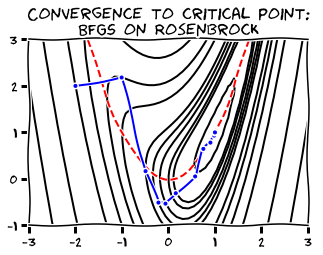
\includegraphics[width=0.65\linewidth]{images/bfgs.png}
\caption{The BFGS method: Rosenbrock function}
\label{figure:BFGS}
\end{figure}
\end{example}